\begin{figure}[tb]
\center
  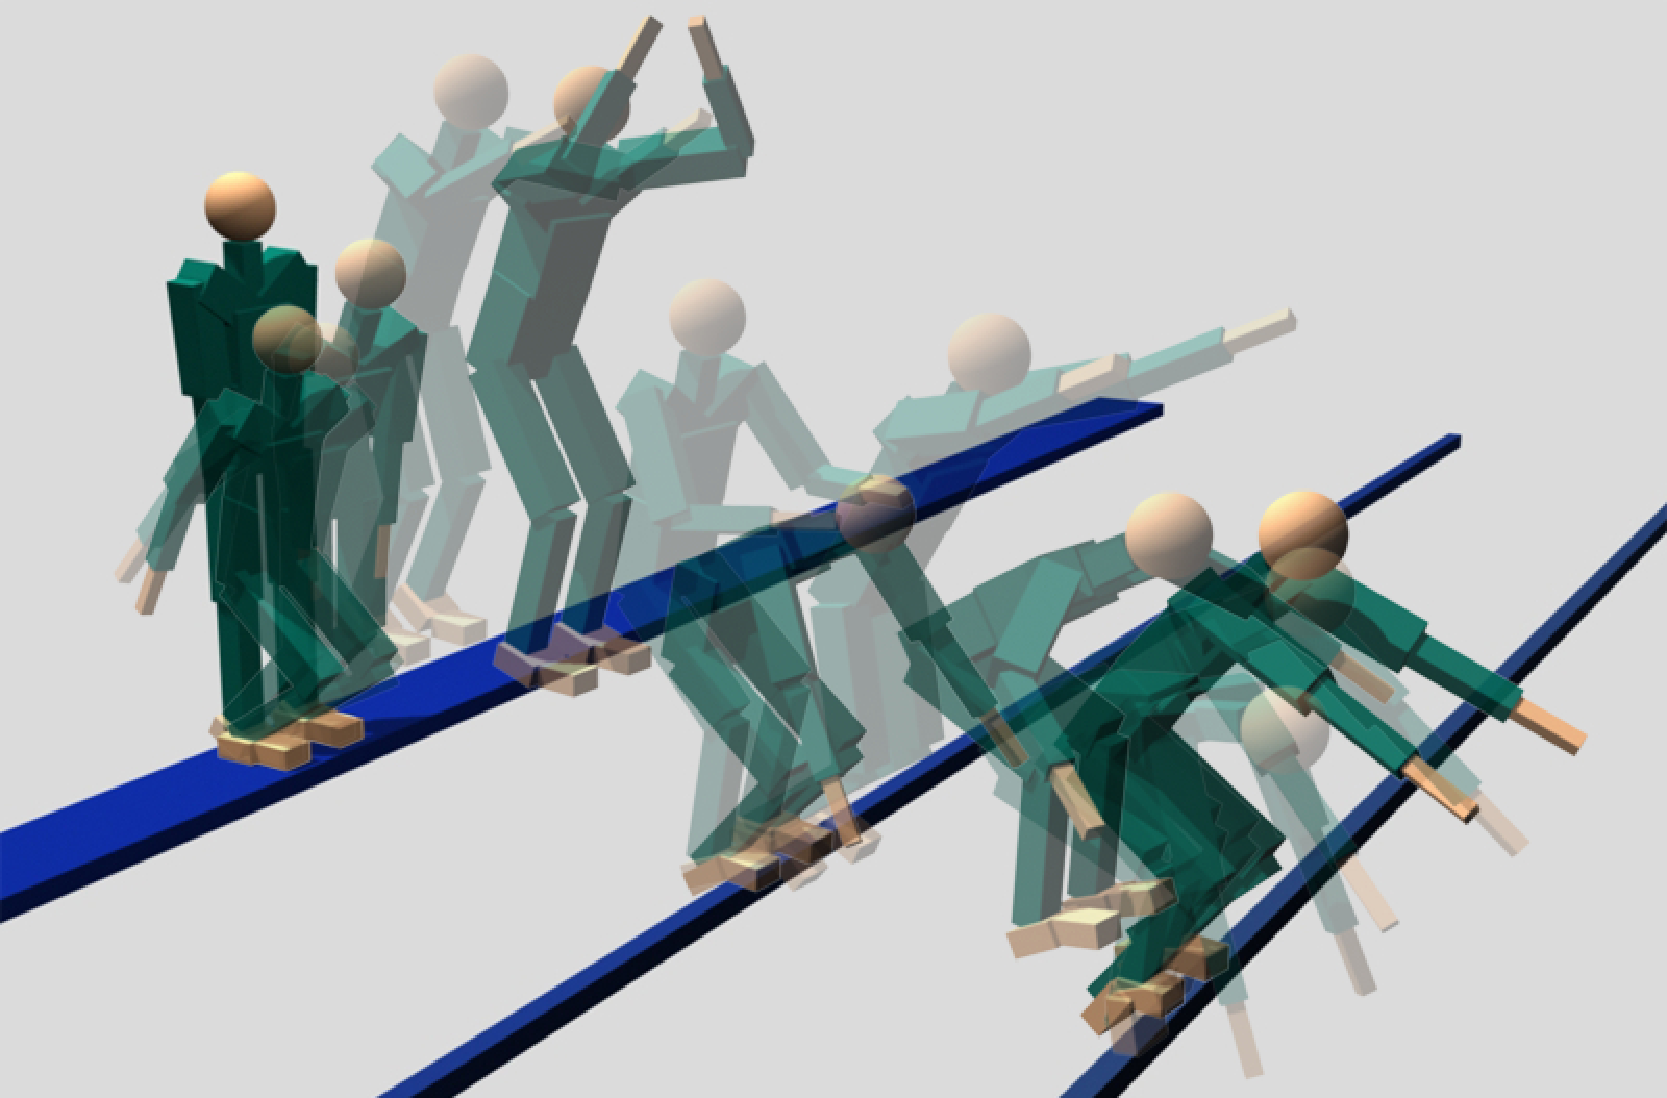
\includegraphics[width=0.7\linewidth]{images/teaser}
  \caption{
  Two precision jumps on narrow rails.
  }
  \label{fig:parkour_teaser}
\end{figure}

\quad
\section{Motivation}

Mastering a dynamic motor skill, such as a handstand in gymnastics, or
a precision jump in Parkour,
usually requires an iterative process
with interactive coaching and repetitive practices. Based on the
current skill level of the trainee, the coach gives instructions that
emphasize the key areas for improvement. The trainee then internalizes
the new information and improves the skill through practices. The
learning process alternates between coaching and practicing stages
until the skill is acquired. In contrast, teaching a physically
simulated character a new motor skill entirely depends on the effort
of the controller developer, from the design of the control
architecture to the tweaking of low-level control parameters. We
hypothesize that the controller development can be greatly simplified
by exploiting the same learning principles humans use to acquire new
motor skills. In addition, if designing new controller can be done in
the similar fashion as coaching a human trainee, the existing
controllers can be easily adapted, extended, or concatenated for new
situations.

This paper attempts to formalize the methodologies humans use to learn
dynamic motor skills. We present an algorithmic framework to
facilitate the iterative learning process of coaching and
practicing. During the coaching stage, the user only needs to provide
a primitive initial controller and
high-level, human-readable instructions as if s/he is coaching a human
trainee. For example, a human coach typically uses high-level
instructions, such as ``extend the legs'' or ``push the ground'', rather
than specific descriptions of joint angles. During the practicing
stage, the character is capable of following the instructions and
improving its motor skill effectively on its own. That is, the
character has the autonomous ability to interpret the abstract
instructions, accumulate the knowledge from the coach, and optimizes
its motion based on the guidance.

The main challenge of this work is to formalize these elusive
principles of human learning into mathematical models for controller
design. Our underlying assumption is that any motor skill can be
achieved by using simple proportion-derivative (PD) style control and
Jacobian transpose control at every actuated joint and every body
part, \emph{if} the control parameters are properly determined. This
formulation, however, introduces a prohibitively large space of
control variables for the existing optimization methods. Our controller
design framework solves this issue by utilizing human coaching
knowledge to select an appropriate subset of control variables
(coaching stage) and relying on a new sampling-based optimization
method to determine the value of control variables (practicing stage).

Using high-level, human-readable instructions can potentially simplify
the controller design, but directly mapping high-level instructions to
low-level control variables is a challenging task. We introduce an
intermediate layer of control module, called control rigs, to
interpret the human instructions during the coaching stage. A control
rig simultaneously controls a set of low-level control variables in a
coordinated fashion. For example, a control rigs flexes legs
uses a single parameter, the distance between the waist and the feet,
to control the target joint angles of the PD controllers on the hips,
knees, and ankles. With this intermediate layer, mapping human
instructions to the low-level control variables can be done
automatically by selecting appropriate control rigs. In addition,
using control rigs instead of low-level variables reduces the search
space for the optimization. We design a set of control rigs from
frequently used instructions for Parkour training. These control rigs
are general and can be reused for coaching different sports.

To determine the control variables efficiently during the practicing
stage, we introduce the concept of ``learning from failure'' using a
sampling-based optimization method. Our key insight is that the failed
samples contain as much useful information as the successful ones. For
example, falling on the ground or hitting obstacles are valuable
experiences to learn vaulting. Instead of throwing away those failed
simulation trials, our algorithm uses them to approximate the boundary
of the feasible region in the control variable space. Having an
approximated feasible region accelerates the optimizations by
preventing the character to repeat failures committed before. Based on
this idea, we build Support Vector Machines in concert with Covariance
Matrix Adaptation (CMA), called Covariance Matrix Adaptation with
Classification (CMA-C). The main advantage of CMA-C is that it
exploits every simulated trial; the successful ones are used to
contract the covariance matrix while the failed ones are used to refine
the boundary of feasible region.

We demonstrate the design process of complex dynamic controllers using
our framework, including precision jumps, turnaround jumps, monkey
vaults, drop-and-rolls, and wall backflips.  We show that the
character started out with basic controllers; using PD control to
track a few roughly specified poses; and were able to learn these
complex dynamic skills within minutes with only a few high-level
instructions from the user. Once a controller is developed,
parameterizing it to a family of similar controllers for concatenation
can be done without additional effort from the user.



